\chapter{検証フレームワーク Actario}
\label{chapter:overview}

本章では、本研究で作成したアクターシステムの検証フレームワーク Actario についての概要を説明する。
Actario では、

\section{概要}

図 \ref{img:overview:workflow} は、Actario を用いてアクターシステムを検証する際のワークフローである。
まず Actario が提供するアクターシステムを記述するための記法を使って、検証したいアクターシステムを記述する。
次にそのアクターシステムが満たしているべき仕様を記述し、それを Actario が提供する証明の機構によって証明する。
最後に Actario が持つ Erlang へのコード抽出機を用いて実装を Erlang に抽出する。

\begin{figure}[tp]
  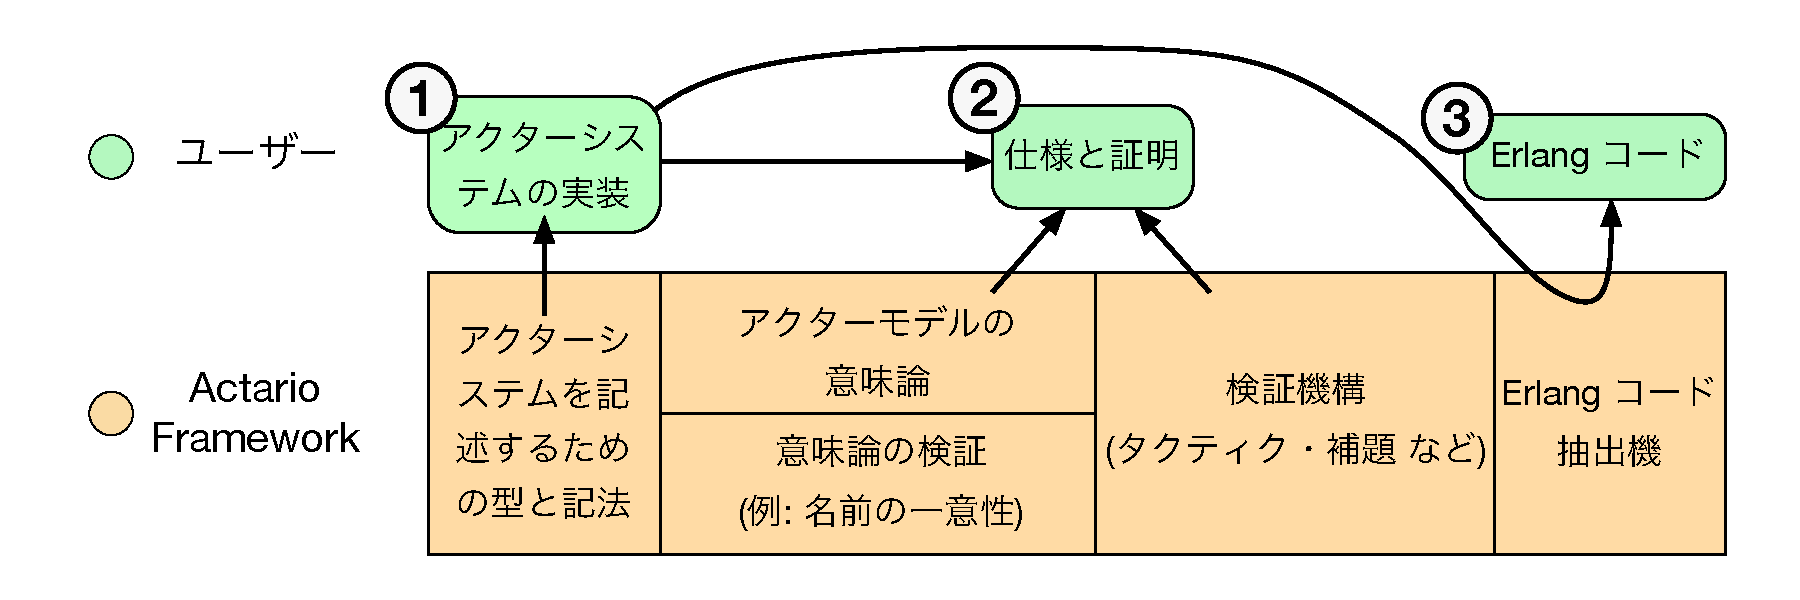
\includegraphics[width=14cm]{./img/workflow.pdf}
  \label{img:overview:workflow}
  \caption{Actario のワークフロー}
\end{figure}

\section{例: 階乗計算アクターシステム}

このアクターシステムは、一つのアクターのなかで階乗を計算するのではなく、
次に何の数を掛けるかという継続を持っているアクターを生成しながら、
階乗を計算する。(?)

\begin{figure}[tp]
  \lstinputlisting{./code/overview/fact.v}
  \label{code:overview:fact}
  \caption{階乗計算アクターシステム}
\end{figure}
